\documentclass[conference]{IEEEtran}
\IEEEoverridecommandlockouts
% The preceding line is only needed to identify funding in the first footnote. If that is unneeded, please comment it out.
\usepackage{cite}
\usepackage{amsmath,amssymb,amsfonts}
\usepackage{algorithmic}
\usepackage{graphicx}
\usepackage{textcomp}
\usepackage{xcolor}
\usepackage[]{algorithm2e}
\def\BibTeX{{\rm B\kern-.05em{\sc i\kern-.025em b}\kern-.08em
    T\kern-.1667em\lower.7ex\hbox{E}\kern-.125emX}}
\begin{document}

\title{Indirect Visual Odometry with Optical Flow}


\author{\IEEEauthorblockN{Chenguang Huang, Andong Tan}
\IEEEauthorblockA{\textit{Department of Mathematics and Informatics} \\
\textit{Technical University of Munich}\\
Munich, Germany \\
chenguang.huang@tum.de, andong.tan@tum.de\\
}
}

\maketitle

\begin{abstract}
   With the increasing need of robotics application in industry...
		
\end{abstract}

\begin{IEEEkeywords}
Optical Flow, Visual Odometry, Computer Vision
\end{IEEEkeywords}


\section{Introduction}
Computer vision related tasks in robotics are attracting more and more attention. One typical task is the visual odometry. It is used widely in applications which require the depth information of objects without directly relying on distance measurement sensors like Lidar. Besides, many applications uses visual odometry to help with the motion planning of some specific agent. Therefore, this function could cause critical problems if it is not reliable. To ensure the safety of the agent, a common choice is to use mathematically provable methods to realize the function rather than using currently unexplainable techniques like deep learning. Thus it worths looking into the implementation details of visual odometry using traditional explainable methods.

To estimate the depth of some specific object, at least two images are needed if there is no prior assumption in how the world is constructed. However, before estimating the depth through triangulation, corresponding point in two images which describes the same 3D point should be found. The first way to achieve this is through key point detection in both images, and find the matching point pairs through similarity comparison. The second way to achieve this is through optical flow, which computes an estimated position of a pixel in the second image according its position in the first image. The above two ways are also suitable to find the point matching pairs between consecutive frames. 

This paper mainly compares the above two methods. 

The following sections are structured as below: Section II presents some basic concepts used in the two methods. Section III describes the pipeline of the two methods. Section IV shows the implementation details. Section V evaluates the difference between these two methods, and Section VI concludes the work.


\section{Basic Concepts}
To understand the methods better, some basic concepts are summarized in this section.

\subsection{Visual Odometry}
Odometry means the estimation of the change in position over time. And visual odometry refers to the estimation of the motion of a camera in real time through sequential images. In the context of vision based navigation, where cameras are often integrated in the robot, visual odometry can be used to estimate the ego motion of the mobile robot, and thus help to build a map in real time around the robot to support the navigation.

\subsection{Optical Flow} The optical flow is apparent 2D motion which is observable between consecutive images. It can also be understood as pixel-wise motion estimation, because the optical flow calculates the motion of a specific pixel between two consecutive frames. Two main types of optical flow calculation are the Lukas \& Kanade method (indirect method) and Horn \& Schunck method (variational method). These two methods have different assumptions but both calculates the optical flow through an optimization process.

In Lukas \& Kanade method, it assumes that (i) the motion is constant in a local neighborhood (ii) the brightness of a specific pixel is constant in different frames. Under the above assumptions, the energy function in the Lukas \& Kanade method is formulated as follows:

\begin{equation}
	E(v) = \int_{W(x)} |\Delta I(x', t)^Tv + I_t(x',t) |^2dx'
\end{equation}

where $I(x',t)$ denotes the brightness of position $x'$ at time $t$ in the image, $I_t$ denotes the derivative of brightness with respect to the time $t$, and $W(x)$ denotes the neighborhood of pixel $x'$. The optical flow $v$ is calculated via the minimization of the above energy function. It generates sparse flow vectors.

In contrast, the Horn \& Schunck method assumes (i) the brightness of a specific pixel is a constant in different frames (ii) the motions are spatially smooth. This method generates dense flow vectors. The energy function of this method is:

\begin{equation}
	E(u,v) = \int\int[(I_xu + I_yv + I_t)^2+\alpha^2(||\Delta u ||^2 + ||\Delta v ||^2)]dxdy
\end{equation} 

where $I_x$ and $T_y$ are the derivatives of brightness with respect to x and y axis, respectively. $u$ and $v$ are velocity in vertical and parallel directions. In the end, optical flow is obtained through solving for $u$ and $v$ variable.		

\subsection{Key Point Detection}
The environment is continuous and complex. To successfully navigate in such en environment, some key information is more important than the other information. In the image, one kind of typical key information is the corner point. 

One usual method to detect such corner points is through the analysis of the gradient of the image \cite{gradient}. Typical methods include Foerstner and Harris detector \cite{detector}. More recently, detectors like BRIEF, SURF, FAST, and Shi-Tomasi are quite popular, and have many extended versions. In our experiment, key point detection is used to extract important information from the image frames to build the map.

\subsection{Point Matching}
To construct a 3D map, the matching relationship of points between frames are important, otherwise it will cause big error in the triangulation and possibly make the optimization process in determining the 3D position of a landmark unable to converge.

Finding matches between point in consecutive frames are typically done through the comparison of descriptors of two points. If the similarity between two descriptors is high enough, the two corresponding points are considered to be different projections of the same real world point. 

One method to compute the descriptor is called the ORB descriptor \cite{orb}. ORB descriptor uses the BRIEF descriptor \cite{brief} and the orientation of the detected key points to represent the feature of a corner point. According to a set of principles, the correspondence of points between frames will be calculated.
  
\section{Structure Design}
P1
\section{Implementation}
P4


\section{Evaluation}
This section evaluates the performance difference between the matching method using optical flow and the matching method fully relying on key point detection, as well as the performance of the optical flow method under different set of hyper parameters. The evaluation focuses on three main aspects: precision, execution time, and visualization.

As described in the previous section, we use a grid to segment the image frame and decide whether the next frame is a key frame. A basic set of parameters for the grid of our experiments are as follows:


\begin{table}[h!]
	\begin{center}
		\caption{Basic set of parameters}
		\label{tab:basicset}
		\begin{tabular}{llll} % <-- Alignments: 1st column left, 2nd middle and 3rd right, with vertical lines in between
			\textbf{Image height (pixel)} & \textbf{Image width (pixel)} & \textbf{Grid size (pixel $\times$ pixel)}& \textbf{Min. number of key points}\\
			$h$ & $w$ & $s$ & $m$ \\
			\hline
			480 & 752 & 32 $\times$ 32 & 100 \\
	
		\end{tabular}
	\end{center}
\end{table}

The grid size is designed to be so such that it's divisible by the image height and width. Besides, we find through experiments that square grids brings higher precision in the following experiments than rectangular grids. Similarly, the minimum number of key points 100 is found through experiments. To simplify the following discussion, we set the grid size and the minimum number of key points to be a constant, and discuss the influence of other hyper parameters in the rest of the section.
%%
%\itemize
%\item  Strategy

%1. Square grid

%2. Add key points in each cell

%3. Use empty cells number to decide next key frame
%%

\subsection{Precision}

\begin{table}
	\centering
	\caption{RMSE precision under different number of Max. empty cells}
	\label{tab:precision}
	\begin{tabular}{llllll}
		Max. number of \\empty cells (\%)  & 0.35 & 0.4 & 0.42 & 0.44& 0.46 \begin{tabular}[c]{@{}l@{}}  \\\end{tabular}  \\
		RMSE  & 0.1303 & 0.1295 & 0.1099&0.1563&0.1304\\
		 & & & & &\\
		Rmse using method \\without optical flow&0.1012 & & & &		                                                
	\end{tabular}
\end{table}

The table \ref{tab:precision} shows how precision measured as Root Mean Square Error (RMSE) changes when the maximum number of empty cells percentage changes. This variable is designed to control the maximum area of the image where there is no key point. When the empty area is too big, it means we losses a lot of information from these areas and our construction of the map could be not precise enough. When this happen, the next frame will be set as a key frame, and key point detection will be executed. 

From the table it is clear that when the maximum number of empty cells percentage is too small or too large, the precision of the built map will decrease. This means, if we do new key points detection too frequently, we would construct the map using too many key points, which means too many noises, as the key point detection itself is also not 100\% precise. However, if we do key point detection too sparsely, we would have too less key points to construct the map, which indicates that even some small noises could cause a big error in map construction and thus cause an increased RMSE value. In the best case, the RMSE will reach a similar value as the method without using optical flow. Figure \ref{fig:max_empty_cell} shows more experiment data in a visualized way.

\begin{figure}
	\label{fig:max_empty_cell}
	\centering
	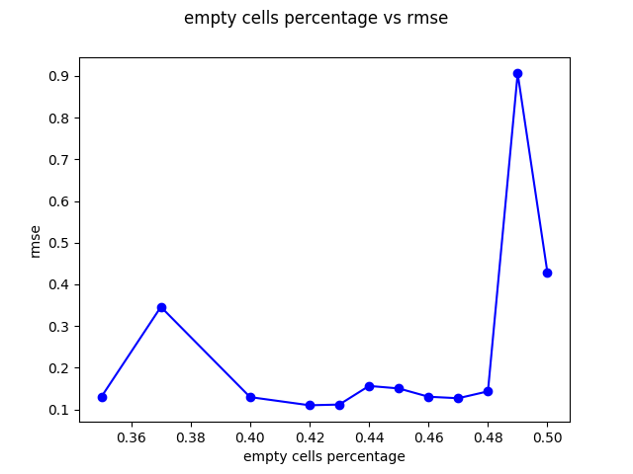
\includegraphics[width=0.5\textwidth]{img/max_num_empty_cell1.png}
	\caption{Visualized version of RMSE change with different parameter of max. number of empty cells percentage}
\end{figure}


\subsection{Execution Time}
The evaluation on execution time includes three parts: detection time, optimization time, and key point matching time. Choosing these three aspects is because: all these three steps are common in two methods, and the difference between these two methods has a big impact on the execution time of these three steps.

%Because the two methods mainly differ in key point detection process, %which influences the optimization time a lot, and the optical flow %method has additionally the optical flow calculation time. Besides, the %optimization step also takes most of the time in the whole %Simultaneously Localization And Mapping (SLAM) process. 

\subsubsection{Detection Time}
The table \ref{tab:detection} shows how detection time changes with change of max number of empty cells percentage. Firstly, it is obvious that the detection time in the method using optical flow is much less than the method without optical flow, because the method using optical flow has replaced a lot of key point detection operation and find the matching points between frames using optical flow. Secondly, it's reasonable to see that with an increasing threshold for maximum empty cells percentage, the detection time generally decreases. This is due to the decreasing frequency of key frames, therefore the detection operation is executed less frequently. The experiment result shows that there is a slight increase on detection time when the threshold is set to 0.44 in comparison to 0.42, we think this could due to the fact that some frames have more textures and corners than the others, and a specific choice of 0.44 occasionally lets us have more key frames in these pictures with a lot of texture and corners. And thus increases the detection time slightly.  

\begin{table}
	\centering
	\caption{Detection time under different number of Max. empty cells percentage}
	\label{tab:detection}
	\begin{tabular}{llllll}
		Max. number of \\empty cells (\%)  & 0.35 & 0.4 & 0.42 & 0.44& 0.46 \begin{tabular}[c]{@{}l@{}}  \\\end{tabular}  \\
		Detection time (s)  & 3.03643
		 & 2.73232
		  & 2.43286&2.62328&2.26326\\
		& & & & &\\
		Detection time using method \\without optical flow&44.0214 & & & &		                                                
	\end{tabular}
\end{table}


\subsubsection{Optimization time}
Optimization takes the most time of the whole pipeline. Here we choose the best parameter for maximum percentage of the number of empty cells, which is 0.42 and compare it with the method without optical flow. The results are shown in table \ref{tab:optimization}.

The optimization time of the optical flow method is much higher than the method fully depending on key point detection. Although the number of landmarks are in similar level, the number of key frames and observation in optical flow method is much higher than the other one, which causes the huge difference in optimization time. As the optimization process only happen in key frames, an increased number of key frames naturally increases the total optimization time. Here comes automatically the question: Why do we have more key frames and observations in optical flow based method?

Firstly, selection of key frames based on counting empty cells (optical flow method) rather than key point number (non optical flow method) in the image leads to a denser choice of key frames. Therefore the number of key frames is much higher.

Secondly, a possible reason for the large number of observations is that our pipeline forces a key point detection operation in every small grid of key frames. Although this has the advantage that the detected key points are more widely distributed in the whole image to help with a preciser optimization process, it has the disadvantage that many noises are also introduced and many noisy points are considered as an observation of some specific landmark.  

The above reasons together leads to the difference in optimization time between two methods.

\begin{table}
	\centering
	\caption{Optimization time comparison}
	\label{tab:optimization}
	\begin{tabular}{lll}
		  & Max. number of empty cells(\%) = 0.42 & Method without optical flow   \\
		Opt. time (s)  & 305.043 & 65.8619\\
		Num. landmarks &290657 &221886\\
		 Num. observation & 1939460 & 559563 \\        
		 Num. key frames & 414 & 170                 
	\end{tabular}
\end{table}


\subsubsection{Key Point Matching Time}
As a replacement of point descriptor comparison between frames, optical flow is used to track the key point between frames. Therefore, we compare the execution time of optical flow and key point matching through descriptors in the following table \ref{tab:matching}:

\begin{table}
	\centering
	\caption{Key point matching time comparison}
	\label{tab:matching}
	\begin{tabular}{ll}
		Point descriptor matching time (s) &5.79\\
		Optical flow calculation (s) & 117.4~143.1   \\              
	\end{tabular}
\end{table}

The optical flow calculation time is much higher than the key point matching using descriptors. This is due to the fact that optical flow calculation includes an optimization process and the result is calculated iteratively, but descriptor comparison is a rather direct method which only needs several basic mathematical operations. Besides, the descriptor used (ORB) is itself also a very efficient and quick method for comparison.


\subsection{Visualization}
A visual comparison can give more intuition for the performance of different methods. 

Comparing the Figure \ref{fig:optical_flow_global} and Figure \ref{fig:key_point_global}, we could find that the detected points using method of optical flow are more uniformly distributed, this is because in the implementation, we force each grid cell of the segmented image to find feature points, which helps to increase the precision of the estimated camera position.

In Figure \ref{fig:optical_flow_desk} and Figure \ref{fig:key_point_desk}, there are two gray lines representing the calibration board in the vertical direction. We could find that the two gray lines in Figure \ref{fig:optical_flow_desk} are closer than Figure \ref{fig:key_point_desk}, which means a better reconstructed map in this area. A real world picture of this area is offered in Figure 
\ref{fig:desk}.

\begin{figure}
	\label{fig:optical_flow_global}
	\centering
	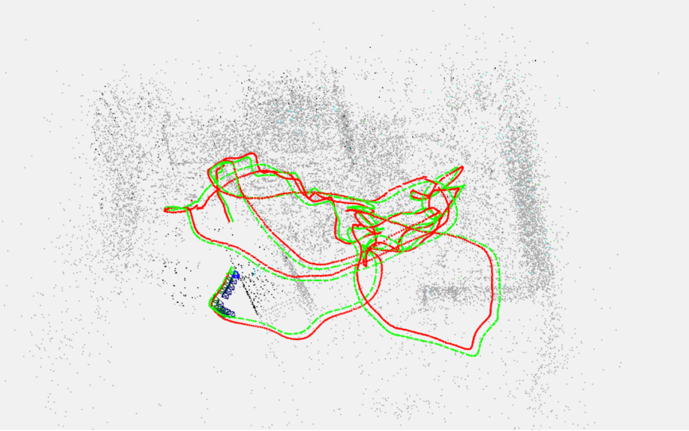
\includegraphics[width=0.5\textwidth]{img/optical_flow_global.png}
	\caption{Ground truth path (red) and calculated path (green) using optical flow based method. Gray points represent detected key points.}
\end{figure}

\begin{figure}
	\label{fig:key_point_global}
	\centering
	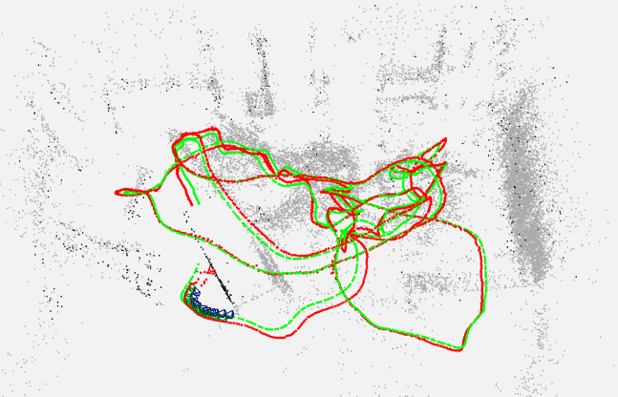
\includegraphics[width=0.5\textwidth]{img/key_point_global.png}
	\caption{Ground truth path (red) and calculated path (green) using method without optical flow. Gray points represent detected key points.}
\end{figure}

\begin{figure}
	\label{fig:optical_flow_desk}
	\centering
	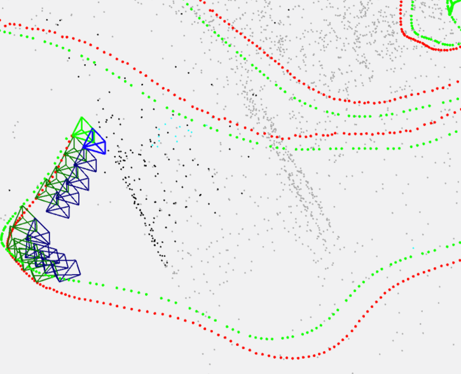
\includegraphics[width=0.5\textwidth]{img/optical_flow_desk.png}
	\caption{Map constructed using optical flow based method. Gray points represent detected key points.}
\end{figure}

\begin{figure}
	\label{fig:key_point_desk}
	\centering
	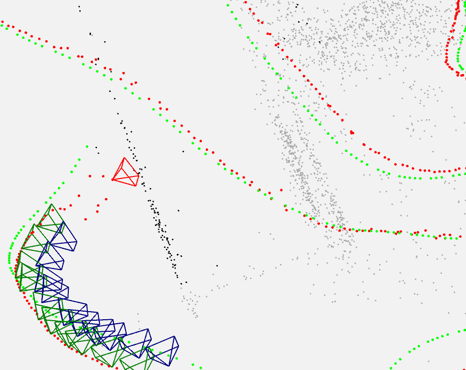
\includegraphics[width=0.5\textwidth]{img/key_point_desk.png}
	\caption{Map constructed using method without optical flow. Gray points represent detected key points.}
\end{figure}


\begin{figure}
	\label{fig:desk}
	\centering
	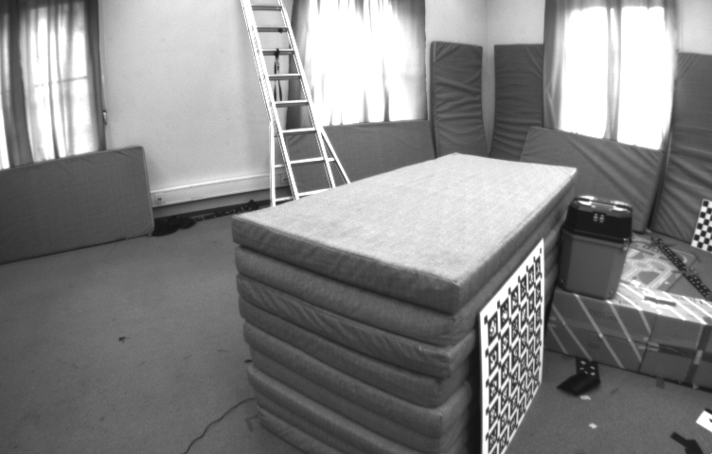
\includegraphics[width=0.5\textwidth]{img/desk.png}
	\caption{The desk image in real world.}
\end{figure}




\section{Conclusion}
P1


\begin{thebibliography}{00}

\bibitem{gradient} H. Wang and M. Brady, “Real-time corner detection algorithm for
motion estimation,” Image and vision computing, vol. 13, no. 9, pp. 695–
703, 1995.

\bibitem{detector} Rodehorst, V.; Koschan, A. Comparison and evaluation of feature point detectors. In Proceedings
of 5th International Symposium Turkish-German Joint Geodetic Days, Technical University of
Berlin, Germany, March, 2006; ISBN 3-9809030-4-4.

\bibitem{orb} E. Rublee, V. Rabaud, K. Konolige, and G. Bradski, “ORB: an efficientalternative  to  SIFT  or  SURF,”  inIEEE  International  Conference  onComputer Vision (ICCV), Barcelona, Spain, November 2011, pp. 2564–2571

\bibitem{brief} E. Rublee, V. Rabaud, K. Konolige and G. Bradski, "ORB: An efficient alternative to SIFT or SURF," 2011 International Conference on Computer Vision, Barcelona, 2011, pp. 2564-2571.



\end{thebibliography}

\end{document}
